\documentclass{article}

\usepackage{fullpage}
\usepackage{amsmath}
\usepackage{amssymb}
\usepackage{amsthm}
\usepackage{graphicx}
\usepackage{xcolor}
\usepackage{hyperref}
\usepackage{tikz}
\usetikzlibrary{arrows.meta, positioning, calc, decorations.pathreplacing, shapes.geometric, fit, backgrounds}
\usepackage{enumitem}
\usepackage{booktabs}
\usepackage{subcaption}
\usepackage{float}

\newtheorem{definition}{Definition}
\newtheorem{remark}{Remark}

% Custom colors
\definecolor{enccolor}{RGB}{66,133,244}
\definecolor{deccolor}{RGB}{234,67,53}
\definecolor{latentcolor}{RGB}{52,168,83}
\definecolor{datacolor}{RGB}{251,188,4}
\definecolor{condcolor}{RGB}{153,51,255}
\definecolor{lightblue}{RGB}{220,235,252}
\definecolor{lightred}{RGB}{252,225,222}
\definecolor{lightgreen}{RGB}{222,247,226}
\definecolor{lightpurple}{RGB}{237,222,252}

\title{
    Variational Autoencoders: \\
    From VAE to Conditional VAE \\[6pt]
    \large A Visual and Mathematical Introduction
}
\author{
    Pan Changxun \\
    2024011323
}
\date{March 2026}

\begin{document}

\maketitle

\begin{abstract}
This note provides a self-contained introduction to the Variational Autoencoder (VAE) and its conditional extension (CVAE). We cover the probabilistic formulation, the evidence lower bound (ELBO), the reparameterization trick, and training procedures for both models, with illustrative diagrams throughout.
\end{abstract}

\tableofcontents
\newpage

%% ============================================================
\section{Background: Latent Variable Models}
%% ============================================================

Many real-world datasets (images, text, audio) lie on low-dimensional manifolds embedded in high-dimensional observation spaces. \emph{Latent variable models} capture this by introducing unobserved variables $z$ that explain the data $x$:
\[
    p_\theta(x) = \int p_\theta(x|z)\,p(z)\,dz.
\]

\begin{figure}[H]
\centering
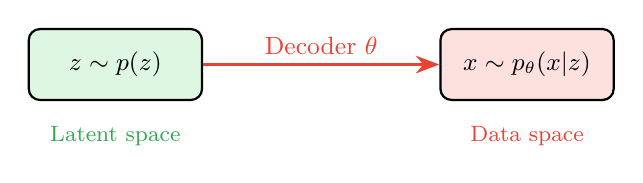
\begin{tikzpicture}[
    >={Stealth[length=3mm]},
    box/.style={draw, rounded corners, minimum width=2.2cm, minimum height=0.9cm, font=\small, thick},
]
    \node[box, fill=lightgreen] (z) {$z \sim p(z)$};
    \node[box, fill=lightred, right=3cm of z] (x) {$x \sim p_\theta(x|z)$};
    \draw[->, thick, deccolor] (z) -- node[above, font=\small] {Decoder $\theta$} (x);
    \node[below=0.2cm of z, font=\footnotesize, latentcolor] {Latent space};
    \node[below=0.2cm of x, font=\footnotesize, deccolor] {Data space};
\end{tikzpicture}
\caption{The generative process: sample $z$ from prior, then generate $x$ via the decoder.}
\label{fig:gen-process}
\end{figure}

The generative story:
\begin{enumerate}
    \item Sample a latent code $z \sim p(z)$ (the \emph{prior}, typically $\mathcal{N}(0,I)$).
    \item Generate data $x \sim p_\theta(x|z)$ (the \emph{decoder / likelihood}).
\end{enumerate}

Two fundamental challenges arise:
\begin{itemize}
    \item \textbf{Intractable marginal likelihood.} $p_\theta(x) = \int p_\theta(x|z)p(z)\,dz$ is intractable when $p_\theta(x|z)$ is a neural network.
    \item \textbf{Intractable posterior.} $p_\theta(z|x) = p_\theta(x|z)p(z)/p_\theta(x)$ requires $p_\theta(x)$.
\end{itemize}

The \textbf{VAE} addresses both via \emph{amortized variational inference}.

%% ============================================================
\section{Variational Autoencoder (VAE)}
%% ============================================================

\subsection{Overall Architecture}

\begin{figure}[H]
\centering
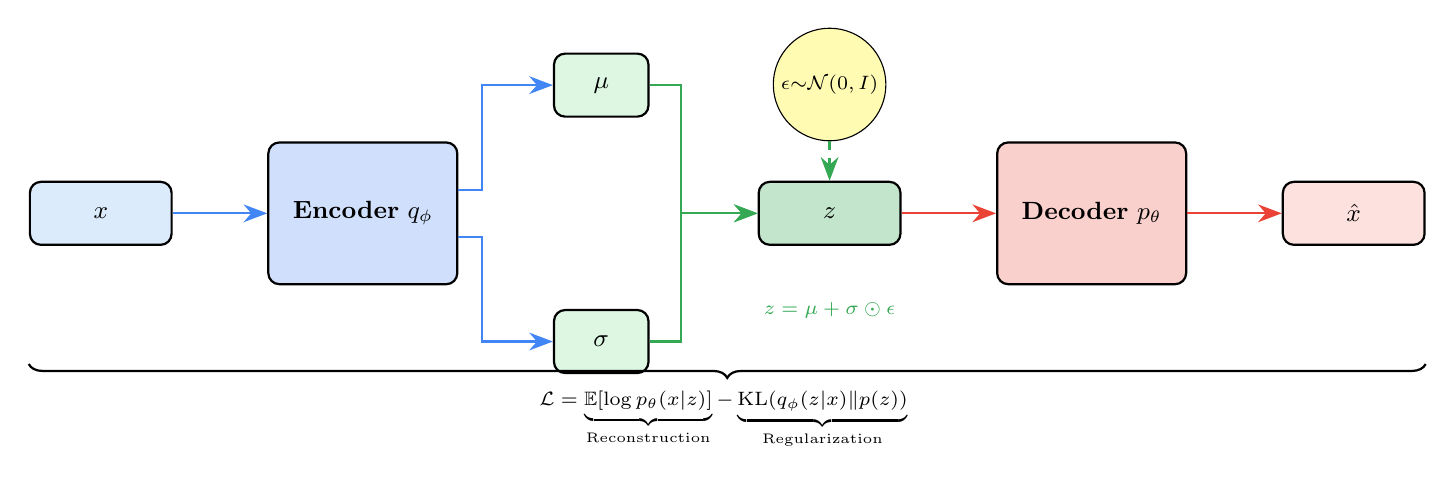
\begin{tikzpicture}[
    >={Stealth[length=3mm]},
    box/.style={draw, rounded corners, minimum width=1.8cm, minimum height=0.8cm, font=\small, thick},
    every node/.style={font=\small},
    node distance=1.2cm,
]
    % Input
    \node[box, fill=lightblue] (input) {$x$};
    % Encoder
    \node[box, fill=enccolor!25, right=1.2cm of input, minimum width=2.4cm, minimum height=1.8cm] (enc) {\textbf{Encoder} $q_\phi$};
    % Mu and Sigma
    \node[box, fill=lightgreen, minimum width=1.2cm, above right=0.3cm and 1.2cm of enc] (mu) {$\mu$};
    \node[box, fill=lightgreen, minimum width=1.2cm, below right=0.3cm and 1.2cm of enc] (sig) {$\sigma$};
    % z
    \node[box, fill=latentcolor!30, right=3.8cm of enc] (z) {$z$};
    % Epsilon
    \node[draw, circle, fill=yellow!30, inner sep=2pt, font=\scriptsize, above=0.5cm of z] (eps) {$\epsilon{\sim}\mathcal{N}(0,I)$};
    % Decoder
    \node[box, fill=deccolor!25, right=1.2cm of z, minimum width=2.4cm, minimum height=1.8cm] (dec) {\textbf{Decoder} $p_\theta$};
    % Output
    \node[box, fill=lightred, right=1.2cm of dec] (output) {$\hat{x}$};

    % Arrows
    \draw[->, thick, enccolor] (input) -- (enc);
    \draw[->, thick, enccolor] (enc.east) ++(0,0.3) -- ++(0.3,0) |- (mu);
    \draw[->, thick, enccolor] (enc.east) ++(0,-0.3) -- ++(0.3,0) |- (sig);
    \draw[->, thick, latentcolor] (mu.east) -- ++(0.4,0) |- (z);
    \draw[->, thick, latentcolor] (sig.east) -- ++(0.4,0) |- (z);
    \draw[->, thick, dashed, latentcolor] (eps) -- (z);
    \draw[->, thick, deccolor] (z) -- (dec);
    \draw[->, thick, deccolor] (dec) -- (output);

    % Annotation
    \node[below=0.6cm of z, font=\scriptsize, align=center, text=latentcolor] {$z = \mu + \sigma \odot \epsilon$};

    % Brace for loss
    \draw[decorate, decoration={brace, amplitude=5pt, mirror}, thick]
        ([yshift=-1.5cm]input.south west) -- ([yshift=-1.5cm]output.south east)
        node[midway, below=6pt, font=\scriptsize, align=center] {
            $\mathcal{L} = \underbrace{\mathbb{E}[\log p_\theta(x|z)]}_{\text{Reconstruction}} - \underbrace{\mathrm{KL}(q_\phi(z|x)\|p(z))}_{\text{Regularization}}$
        };
\end{tikzpicture}
\caption{VAE architecture. The encoder maps $x$ to distribution parameters $(\mu, \sigma)$. A latent code $z$ is sampled via the reparameterization trick. The decoder reconstructs $\hat{x}$ from $z$. Training maximizes the ELBO.}
\label{fig:vae-arch}
\end{figure}

\subsection{Model Specification}

\begin{center}
\renewcommand{\arraystretch}{1.4}
\begin{tabular}{lll}
\toprule
\textbf{Component} & \textbf{Distribution} & \textbf{Role} \\
\midrule
Prior & $p(z) = \mathcal{N}(z; 0, I)$ & Latent space structure \\
Decoder & $p_\theta(x|z)$ & Maps latent codes to data \\
Encoder & $q_\phi(z|x) = \mathcal{N}(z;\mu_\phi(x), \mathrm{diag}(\sigma^2_\phi(x)))$ & Approximates posterior \\
\bottomrule
\end{tabular}
\end{center}

\subsection{Evidence Lower Bound (ELBO)}

Since $\log p_\theta(x)$ is intractable, we derive a tractable lower bound.

\begin{figure}[H]
\centering
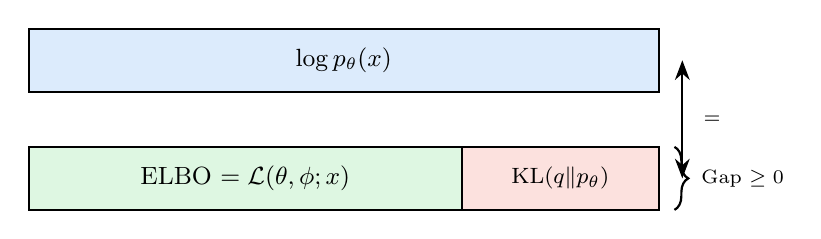
\begin{tikzpicture}[
    >={Stealth[length=2.5mm]},
    every node/.style={font=\small},
]
    % Bar representing log p(x)
    \fill[lightblue] (0,0) rectangle (8,0.8);
    \draw[thick] (0,0) rectangle (8,0.8);
    \node at (4,0.4) {$\log p_\theta(x)$};

    % ELBO part
    \fill[lightgreen] (0,-1.5) rectangle (5.5,-0.7);
    \draw[thick] (0,-1.5) rectangle (5.5,-0.7);
    \node at (2.75,-1.1) {ELBO $= \mathcal{L}(\theta,\phi;x)$};

    % KL gap
    \fill[lightred] (5.5,-1.5) rectangle (8,-0.7);
    \draw[thick] (5.5,-1.5) rectangle (8,-0.7);
    \node at (6.75,-1.1) {\footnotesize $\mathrm{KL}(q\|p_\theta)$};

    % Brace
    \draw[decorate, decoration={brace, amplitude=5pt}, thick]
        (8.2,-0.7) -- (8.2,-1.5) node[midway, right=6pt, font=\scriptsize, align=left] {Gap $\geq 0$};

    % Equality
    \draw[<->, thick] (8.3,0.4) -- (8.3,-1.1) node[midway, right=4pt, font=\scriptsize] {$=$};
\end{tikzpicture}
\caption{Decomposition: $\log p_\theta(x) = \text{ELBO} + \mathrm{KL}(q_\phi(z|x)\|p_\theta(z|x))$. Since $\mathrm{KL} \geq 0$, the ELBO is a lower bound.}
\label{fig:elbo-decomp}
\end{figure}

\begin{align}
\log p_\theta(x)
&= \log \int p_\theta(x,z)\,dz \nonumber \\
&= \log \int q_\phi(z|x) \frac{p_\theta(x,z)}{q_\phi(z|x)}\,dz \nonumber \\
&\geq \int q_\phi(z|x) \log \frac{p_\theta(x,z)}{q_\phi(z|x)}\,dz \qquad \text{(Jensen's inequality)} \nonumber \\
&= \mathbb{E}_{q_\phi(z|x)}\!\left[\log p_\theta(x|z)\right] - \mathrm{KL}\!\left(q_\phi(z|x) \,\|\, p(z)\right). \label{eq:elbo}
\end{align}

\[
\boxed{
    \mathcal{L}(\theta, \phi; x) = \underbrace{\mathbb{E}_{q_\phi(z|x)}[\log p_\theta(x|z)]}_{\text{Reconstruction}} - \underbrace{\mathrm{KL}(q_\phi(z|x) \| p(z))}_{\text{Regularization}}
}
\]

Precisely, we have:
\[
    \log p_\theta(x) = \mathcal{L}(\theta,\phi;x) + \mathrm{KL}(q_\phi(z|x) \| p_\theta(z|x)) \geq \mathcal{L}(\theta,\phi;x).
\]

\paragraph{Interpretation of each term (Figure~\ref{fig:elbo-terms}).}

\begin{figure}[H]
\centering
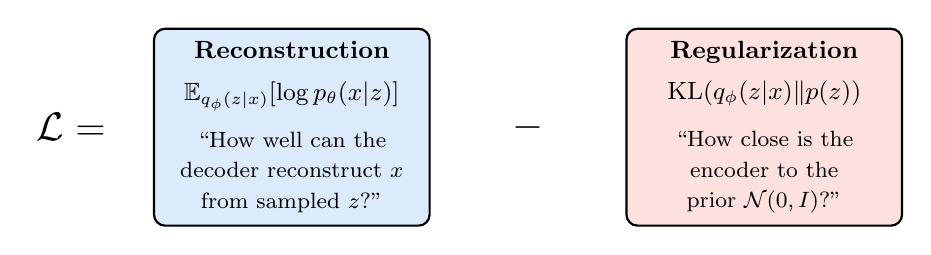
\begin{tikzpicture}[
    >={Stealth[length=2.5mm]},
    termbox/.style={draw, rounded corners, thick, minimum width=3.5cm, minimum height=2.5cm, align=center, font=\small},
]
    \node[termbox, fill=lightblue] (recon) at (0,0) {
        \textbf{Reconstruction}\\[4pt]
        $\mathbb{E}_{q_\phi(z|x)}[\log p_\theta(x|z)]$\\[6pt]
        \footnotesize ``How well can the\\
        \footnotesize decoder reconstruct $x$\\
        \footnotesize from sampled $z$?''
    };
    \node[font=\Large] at (3,0) {$-$};
    \node[termbox, fill=lightred] (kl) at (6,0) {
        \textbf{Regularization}\\[4pt]
        $\mathrm{KL}(q_\phi(z|x)\|p(z))$\\[6pt]
        \footnotesize ``How close is the\\
        \footnotesize encoder to the\\
        \footnotesize prior $\mathcal{N}(0,I)$?''
    };
    \node[font=\Large] at (-2.8,0) {$\mathcal{L} =$};
\end{tikzpicture}
\caption{The two terms of the ELBO and their intuitive meanings.}
\label{fig:elbo-terms}
\end{figure}

\subsection{The Reparameterization Trick}

To optimize the ELBO via gradient descent, we need gradients w.r.t.\ $\phi$. However, $\mathbb{E}_{q_\phi(z|x)}[\cdot]$ involves sampling from a $\phi$-dependent distribution.

\begin{figure}[H]
\centering
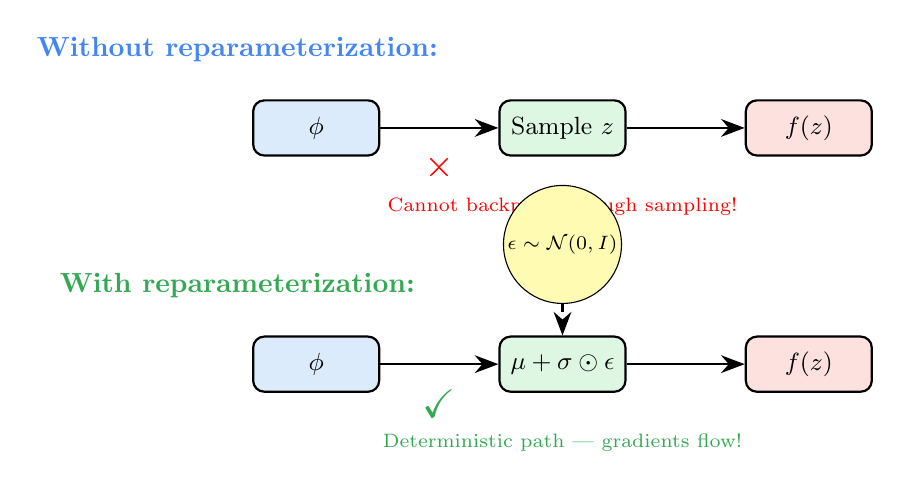
\begin{tikzpicture}[
    >={Stealth[length=3mm]},
    box/.style={draw, rounded corners, minimum width=1.6cm, minimum height=0.7cm, font=\small, thick},
    every node/.style={font=\small},
]
    % Without trick
    \node[font=\bfseries, enccolor] at (-1, 2) {Without reparameterization:};
    \node[box, fill=lightblue] (phi1) at (0,1) {$\phi$};
    \node[box, fill=lightgreen, right=1.5cm of phi1] (sample1) {Sample $z$};
    \node[box, fill=lightred, right=1.5cm of sample1] (f1) {$f(z)$};
    \draw[->, thick] (phi1) -- (sample1);
    \draw[->, thick] (sample1) -- (f1);
    \node[red, font=\Large] at ($(phi1)!0.5!(sample1) + (0,-0.5)$) {\texttimes};
    \node[red, font=\scriptsize, below=0.4cm of sample1] {Cannot backprop through sampling!};

    % With trick
    \node[font=\bfseries, latentcolor] at (-1, -1) {With reparameterization:};
    \node[box, fill=lightblue] (phi2) at (0,-2) {$\phi$};
    \node[box, fill=lightgreen, right=1.5cm of phi2] (determ) {$\mu + \sigma \odot \epsilon$};
    \node[box, fill=lightred, right=1.5cm of determ] (f2) {$f(z)$};
    \node[draw, circle, fill=yellow!30, inner sep=1pt, font=\scriptsize, above=0.4cm of determ] (eps2) {$\epsilon \sim \mathcal{N}(0,I)$};
    \draw[->, thick] (phi2) -- (determ);
    \draw[->, thick] (determ) -- (f2);
    \draw[->, thick, dashed] (eps2) -- (determ);
    \node[latentcolor, font=\Large] at ($(phi2)!0.5!(determ) + (0,-0.5)$) {\checkmark};
    \node[latentcolor, font=\scriptsize, below=0.4cm of determ] {Deterministic path --- gradients flow!};
\end{tikzpicture}
\caption{The reparameterization trick moves stochasticity to an external noise variable $\epsilon$, creating a differentiable path from $\phi$ to $z$.}
\label{fig:reparam}
\end{figure}

The trick expresses $z$ as a deterministic, differentiable function of $\phi$:
\[
    z = \mu_\phi(x) + \sigma_\phi(x) \odot \epsilon, \qquad \epsilon \sim \mathcal{N}(0, I).
\]
Now gradients w.r.t.\ $\phi$ flow through $\mu_\phi$ and $\sigma_\phi$ via standard backpropagation.

\subsection{Closed-Form KL for Gaussians}

When $q_\phi(z|x) = \mathcal{N}(\mu, \mathrm{diag}(\sigma^2))$ and $p(z) = \mathcal{N}(0, I)$ with $z \in \mathbb{R}^d$:
\[
    \mathrm{KL}(q_\phi(z|x) \| p(z)) = \frac{1}{2}\sum_{j=1}^{d}\left(\mu_j^2 + \sigma_j^2 - 1 - \log \sigma_j^2\right).
\]

\subsection{Graphical Model}

\begin{figure}[H]
\centering
\begin{subfigure}[b]{0.4\textwidth}
\centering
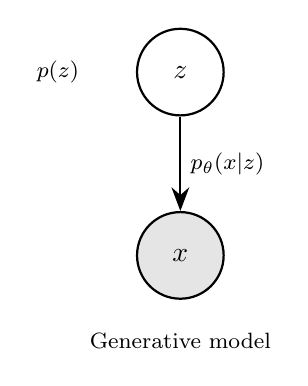
\begin{tikzpicture}[
    >={Stealth[length=3mm]},
    obs/.style={draw, circle, thick, minimum size=1.1cm, fill=gray!20},
    lat/.style={draw, circle, thick, minimum size=1.1cm, fill=white},
]
    \node[lat] (z) {$z$};
    \node[obs, below=1.2cm of z] (x) {$x$};
    \draw[->, thick] (z) -- node[right, font=\footnotesize] {$p_\theta(x|z)$} (x);
    \node[left=0.6cm of z, font=\footnotesize] {$p(z)$};
    \node[below=0.3cm of x, font=\footnotesize] {Generative model};
\end{tikzpicture}
\caption{Generative model $p_\theta$}
\end{subfigure}
\hfill
\begin{subfigure}[b]{0.4\textwidth}
\centering
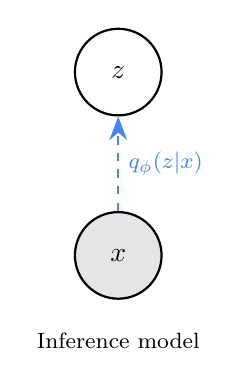
\begin{tikzpicture}[
    >={Stealth[length=3mm]},
    obs/.style={draw, circle, thick, minimum size=1.1cm, fill=gray!20},
    lat/.style={draw, circle, thick, minimum size=1.1cm, fill=white},
]
    \node[obs] (x) {$x$};
    \node[lat, above=1.2cm of x] (z) {$z$};
    \draw[->, thick, enccolor, dashed] (x) -- node[right, font=\footnotesize] {$q_\phi(z|x)$} (z);
    \node[below=0.3cm of x, font=\footnotesize] {Inference model};
\end{tikzpicture}
\caption{Inference model $q_\phi$}
\end{subfigure}
\caption{Graphical models for VAE. Shaded nodes are observed; unshaded are latent. (a)~The generative model defines $p(z)p_\theta(x|z)$. (b)~The inference model (encoder) approximates $p_\theta(z|x)$.}
\label{fig:vae-graphical}
\end{figure}

\subsection{Training Algorithm}

\begin{center}
\fbox{\parbox{0.92\textwidth}{
\textbf{Algorithm 1: VAE Training}\\[4pt]
\textbf{Input:} Dataset $\mathcal{D} = \{x^{(1)}, \ldots, x^{(N)}\}$, learning rate $\eta$\\[2pt]
\textbf{Repeat} until convergence:
\begin{enumerate}[leftmargin=1.5em, itemsep=1pt, topsep=2pt]
    \item Sample mini-batch $\{x^{(i)}\}_{i=1}^{M}$ from $\mathcal{D}$
    \item \textbf{For} each $x^{(i)}$ in mini-batch:
    \begin{enumerate}[label=(\alph*), leftmargin=1.5em, itemsep=1pt]
        \item \textbf{Encode}: $\mu^{(i)}, \sigma^{(i)} \leftarrow \text{Encoder}_\phi(x^{(i)})$
        \item \textbf{Sample}: $\epsilon^{(i)} \sim \mathcal{N}(0,I)$;\; $z^{(i)} = \mu^{(i)} + \sigma^{(i)} \odot \epsilon^{(i)}$
        \item \textbf{Decode}: Compute $\log p_\theta(x^{(i)}|z^{(i)})$
        \item \textbf{KL}: $D_i = \frac{1}{2}\sum_j\!\left((\mu_j^{(i)})^2 + (\sigma_j^{(i)})^2 - 1 - \log(\sigma_j^{(i)})^2\right)$
    \end{enumerate}
    \item $\mathcal{L} \leftarrow \frac{1}{M}\sum_{i=1}^{M}\left[\log p_\theta(x^{(i)}|z^{(i)}) - D_i\right]$
    \item $\theta, \phi \leftarrow \theta, \phi + \eta \nabla_{\theta,\phi} \mathcal{L}$ \quad (e.g., Adam)
\end{enumerate}
}}
\end{center}

\subsection{Generation (Sampling)}

After training:
\begin{enumerate}
    \item Sample $z \sim \mathcal{N}(0, I)$.
    \item Compute $\hat{x} = \mu_\theta(z)$ (or sample $\hat{x} \sim p_\theta(x|z)$).
\end{enumerate}

\begin{figure}[H]
\centering
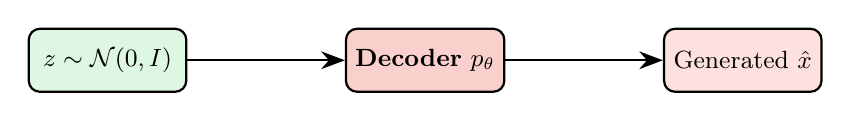
\begin{tikzpicture}[
    >={Stealth[length=3mm]},
    box/.style={draw, rounded corners, minimum width=2cm, minimum height=0.8cm, font=\small, thick},
]
    \node[box, fill=lightgreen] (prior) {$z \sim \mathcal{N}(0,I)$};
    \node[box, fill=deccolor!25, right=2cm of prior] (dec) {\textbf{Decoder} $p_\theta$};
    \node[box, fill=lightred, right=2cm of dec] (gen) {Generated $\hat{x}$};
    \draw[->, thick] (prior) -- (dec);
    \draw[->, thick] (dec) -- (gen);
\end{tikzpicture}
\caption{Generation with a trained VAE: sample from prior, then decode.}
\label{fig:vae-gen}
\end{figure}

%% ============================================================
\section{Conditional VAE (CVAE)}
%% ============================================================

\subsection{Motivation}

The standard VAE models $p(x)$. In many applications, we want $p(x|c)$ where $c$ is a \emph{condition}:
\begin{itemize}
    \item Generate handwritten digits conditioned on class $c \in \{0,\ldots,9\}$.
    \item Generate face images conditioned on attributes.
    \item Predict multiple plausible futures conditioned on context.
\end{itemize}

\begin{figure}[H]
\centering
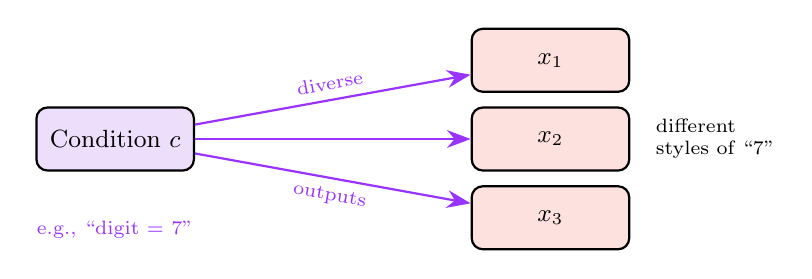
\begin{tikzpicture}[
    >={Stealth[length=3mm]},
    box/.style={draw, rounded corners, minimum width=2cm, minimum height=0.8cm, font=\small, thick},
]
    \node[box, fill=lightpurple] (cond) {Condition $c$};
    \node[box, fill=lightred, right=3.5cm of cond, yshift=1cm] (x1) {$x_1$};
    \node[box, fill=lightred, right=3.5cm of cond, yshift=0cm] (x2) {$x_2$};
    \node[box, fill=lightred, right=3.5cm of cond, yshift=-1cm] (x3) {$x_3$};
    \draw[->, thick, condcolor] (cond) -- node[above, font=\scriptsize, sloped] {diverse} (x1);
    \draw[->, thick, condcolor] (cond) -- (x2);
    \draw[->, thick, condcolor] (cond) -- node[below, font=\scriptsize, sloped] {outputs} (x3);
    \node[below=0.5cm of cond, font=\scriptsize, condcolor] {e.g., ``digit = 7''};
    \node[right=0.2cm of x2, font=\scriptsize, align=left] {different\\styles of ``7''};
\end{tikzpicture}
\caption{CVAE generates diverse outputs $x$ given a condition $c$. The latent variable $z$ captures the variation not explained by $c$.}
\label{fig:cvae-motivation}
\end{figure}

\subsection{Overall Architecture}

\begin{figure}[H]
\centering
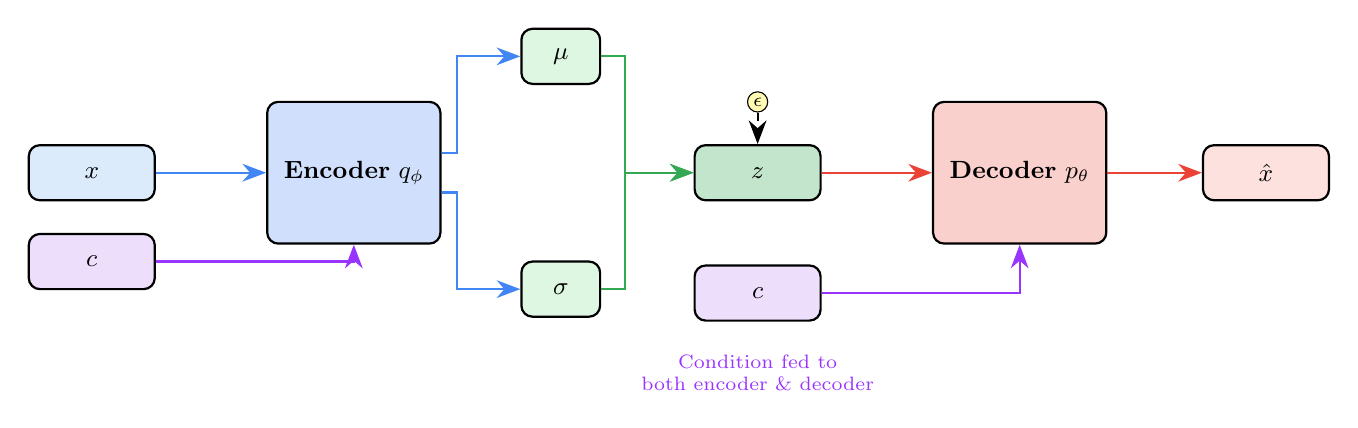
\begin{tikzpicture}[
    >={Stealth[length=3mm]},
    box/.style={draw, rounded corners, minimum width=1.6cm, minimum height=0.7cm, font=\small, thick},
    every node/.style={font=\small},
    node distance=1cm,
]
    % Input x
    \node[box, fill=lightblue] (input) {$x$};
    % Condition c (for encoder)
    \node[box, fill=lightpurple, below=0.4cm of input] (c_enc) {$c$};

    % Encoder
    \node[box, fill=enccolor!25, right=1.4cm of input, minimum width=2.2cm, minimum height=1.8cm] (enc) {\textbf{Encoder} $q_\phi$};

    % Mu and Sigma
    \node[box, fill=lightgreen, minimum width=1cm, above right=0.2cm and 1cm of enc] (mu) {$\mu$};
    \node[box, fill=lightgreen, minimum width=1cm, below right=0.2cm and 1cm of enc] (sig) {$\sigma$};

    % z
    \node[box, fill=latentcolor!30, right=3.2cm of enc] (z) {$z$};

    % Epsilon
    \node[draw, circle, fill=yellow!30, inner sep=1pt, font=\scriptsize, above=0.4cm of z] (eps) {$\epsilon$};

    % Condition c (for decoder)
    \node[box, fill=lightpurple, below=0.8cm of z] (c_dec) {$c$};

    % Decoder
    \node[box, fill=deccolor!25, right=1.4cm of z, minimum width=2.2cm, minimum height=1.8cm] (dec) {\textbf{Decoder} $p_\theta$};

    % Output
    \node[box, fill=lightred, right=1.2cm of dec] (output) {$\hat{x}$};

    % Encoder arrows
    \draw[->, thick, enccolor] (input) -- (enc);
    \draw[->, thick, condcolor] (c_enc) -| (enc);
    \draw[->, thick, enccolor] (enc.east) ++(0,0.25) -- ++(0.2,0) |- (mu);
    \draw[->, thick, enccolor] (enc.east) ++(0,-0.25) -- ++(0.2,0) |- (sig);

    % Sampling arrows
    \draw[->, thick, latentcolor] (mu.east) -- ++(0.3,0) |- (z);
    \draw[->, thick, latentcolor] (sig.east) -- ++(0.3,0) |- (z);
    \draw[->, thick, dashed] (eps) -- (z);

    % Decoder arrows
    \draw[->, thick, deccolor] (z) -- (dec);
    \draw[->, thick, condcolor] (c_dec) -| (dec);
    \draw[->, thick, deccolor] (dec) -- (output);

    % Annotation
    \node[below=0.3cm of c_dec, font=\scriptsize, condcolor, align=center] {Condition fed to\\both encoder \& decoder};
\end{tikzpicture}
\caption{CVAE architecture. Both encoder and decoder receive the condition $c$ as additional input. The encoder is $q_\phi(z|x,c)$ and the decoder is $p_\theta(x|z,c)$.}
\label{fig:cvae-arch}
\end{figure}

\subsection{Model Specification}

\begin{center}
\renewcommand{\arraystretch}{1.4}
\begin{tabular}{lll}
\toprule
\textbf{Component} & \textbf{Distribution} & \textbf{Role} \\
\midrule
Conditional prior & $p_\alpha(z|c)$ or simply $\mathcal{N}(0,I)$ & Latent structure given condition \\
Conditional decoder & $p_\theta(x|z, c)$ & Generates data from $z$ + condition \\
Conditional encoder & $q_\phi(z|x, c)$ & Infers latent code from data + condition \\
\bottomrule
\end{tabular}
\end{center}

\begin{remark}
A common simplification is $p(z|c) = p(z) = \mathcal{N}(0,I)$. A \emph{learned} conditional prior $p_\alpha(z|c) = \mathcal{N}(\mu_\alpha(c), \mathrm{diag}(\sigma^2_\alpha(c)))$ is more expressive and allows different conditions to occupy different latent regions.
\end{remark}

\subsection{ELBO Derivation for CVAE}

All distributions are conditioned on $c$:

\begin{align}
\log p_\theta(x|c)
&= \log \int p_\theta(x|z,c)\,p_\alpha(z|c)\,dz \nonumber \\
&\geq \mathbb{E}_{q_\phi(z|x,c)}\!\left[\log p_\theta(x|z,c)\right] - \mathrm{KL}\!\left(q_\phi(z|x,c) \,\|\, p_\alpha(z|c)\right). \label{eq:cvae-elbo}
\end{align}

\[
\boxed{
    \mathcal{L}_{\mathrm{CVAE}}(\theta,\phi,\alpha; x, c)
    = \underbrace{\mathbb{E}_{q_\phi(z|x,c)}[\log p_\theta(x|z,c)]}_{\text{Conditional reconstruction}}
    - \underbrace{\mathrm{KL}(q_\phi(z|x,c) \| p_\alpha(z|c))}_{\text{Conditional regularization}}
}
\]

\begin{figure}[H]
\centering
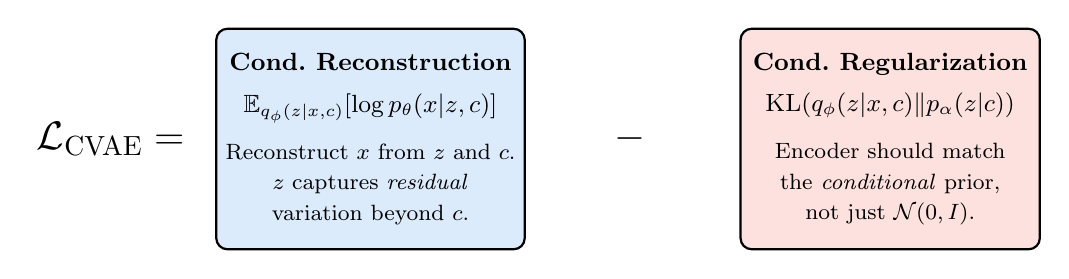
\begin{tikzpicture}[
    >={Stealth[length=2.5mm]},
    termbox/.style={draw, rounded corners, thick, minimum width=3.8cm, minimum height=2.8cm, align=center, font=\small},
]
    \node[termbox, fill=lightblue] (recon) at (0,0) {
        \textbf{Cond.\ Reconstruction}\\[4pt]
        $\mathbb{E}_{q_\phi(z|x,c)}[\log p_\theta(x|z,c)]$\\[6pt]
        \footnotesize Reconstruct $x$ from $z$ and $c$.\\
        \footnotesize $z$ captures \emph{residual}\\
        \footnotesize variation beyond $c$.
    };
    \node[font=\Large] at (3.3,0) {$-$};
    \node[termbox, fill=lightred] (kl) at (6.6,0) {
        \textbf{Cond.\ Regularization}\\[4pt]
        $\mathrm{KL}(q_\phi(z|x,c)\|p_\alpha(z|c))$\\[6pt]
        \footnotesize Encoder should match\\
        \footnotesize the \emph{conditional} prior,\\
        \footnotesize not just $\mathcal{N}(0,I)$.
    };
    \node[font=\Large] at (-3.3,0) {$\mathcal{L}_\mathrm{CVAE} =$};
\end{tikzpicture}
\caption{The two terms of the CVAE ELBO.}
\label{fig:cvae-elbo-terms}
\end{figure}

\subsection{Graphical Model}

\begin{figure}[H]
\centering
\begin{subfigure}[b]{0.4\textwidth}
\centering
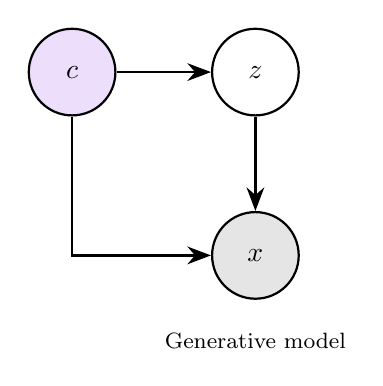
\begin{tikzpicture}[
    >={Stealth[length=3mm]},
    obs/.style={draw, circle, thick, minimum size=1.1cm, fill=gray!20},
    lat/.style={draw, circle, thick, minimum size=1.1cm, fill=white},
    cond/.style={draw, circle, thick, minimum size=1.1cm, fill=lightpurple},
]
    \node[cond] (c) {$c$};
    \node[lat, right=1.2cm of c] (z) {$z$};
    \node[obs, below=1.2cm of z] (x) {$x$};
    \draw[->, thick] (c) -- (z);
    \draw[->, thick] (z) -- (x);
    \draw[->, thick] (c) |- (x);
    \node[below=0.3cm of x, font=\footnotesize] {Generative model};
\end{tikzpicture}
\caption{$p_\alpha(z|c)\,p_\theta(x|z,c)$}
\end{subfigure}
\hfill
\begin{subfigure}[b]{0.4\textwidth}
\centering
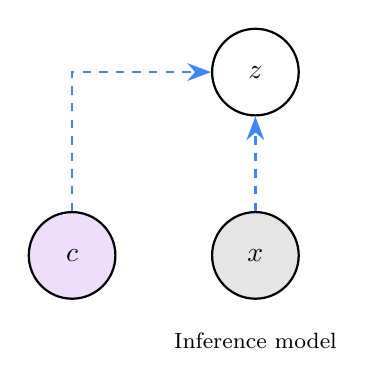
\begin{tikzpicture}[
    >={Stealth[length=3mm]},
    obs/.style={draw, circle, thick, minimum size=1.1cm, fill=gray!20},
    lat/.style={draw, circle, thick, minimum size=1.1cm, fill=white},
    cond/.style={draw, circle, thick, minimum size=1.1cm, fill=lightpurple},
]
    \node[cond] (c) {$c$};
    \node[obs, right=1.2cm of c] (x) {$x$};
    \node[lat, above=1.2cm of x] (z) {$z$};
    \draw[->, thick, enccolor, dashed] (x) -- (z);
    \draw[->, thick, enccolor, dashed] (c) |- (z);
    \node[below=0.3cm of x, font=\footnotesize] {Inference model};
\end{tikzpicture}
\caption{$q_\phi(z|x,c)$}
\end{subfigure}
\caption{Graphical models for CVAE. Purple nodes are conditions (always observed); gray nodes are observed data; white nodes are latent.}
\label{fig:cvae-graphical}
\end{figure}

\subsection{Training Algorithm}

\begin{center}
\fbox{\parbox{0.92\textwidth}{
\textbf{Algorithm 2: CVAE Training}\\[4pt]
\textbf{Input:} Dataset $\{(x^{(i)}, c^{(i)})\}_{i=1}^{N}$, learning rate $\eta$\\[2pt]
\textbf{Repeat} until convergence:
\begin{enumerate}[leftmargin=1.5em, itemsep=1pt, topsep=2pt]
    \item Sample mini-batch $\{(x^{(i)}, c^{(i)})\}_{i=1}^{M}$
    \item \textbf{For} each $(x^{(i)}, c^{(i)})$ in mini-batch:
    \begin{enumerate}[label=(\alph*), leftmargin=1.5em, itemsep=1pt]
        \item \textbf{Encode}: $\mu^{(i)}, \sigma^{(i)} \leftarrow \text{Encoder}_\phi(x^{(i)}, c^{(i)})$
        \item \textbf{Sample}: $z^{(i)} = \mu^{(i)} + \sigma^{(i)} \odot \epsilon^{(i)},\; \epsilon^{(i)} \sim \mathcal{N}(0,I)$
        \item \textbf{Decode}: Compute $\log p_\theta(x^{(i)}|z^{(i)}, c^{(i)})$
        \item \textbf{KL}: Compute $\mathrm{KL}(q_\phi(z|x^{(i)},c^{(i)}) \| p_\alpha(z|c^{(i)}))$
    \end{enumerate}
    \item $\mathcal{L} \leftarrow \frac{1}{M}\sum_{i}\left[\log p_\theta(x^{(i)}|z^{(i)},c^{(i)}) - \mathrm{KL}(\cdots)\right]$
    \item Update $\theta, \phi, \alpha \leftarrow \theta, \phi, \alpha + \eta\,\nabla\mathcal{L}$
\end{enumerate}
}}
\end{center}

\subsection{Conditional Generation}

\begin{figure}[H]
\centering
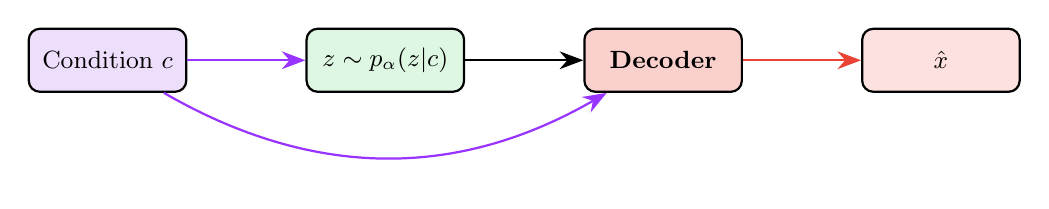
\begin{tikzpicture}[
    >={Stealth[length=3mm]},
    box/.style={draw, rounded corners, minimum width=2cm, minimum height=0.8cm, font=\small, thick},
]
    \node[box, fill=lightpurple] (cond) {Condition $c$};
    \node[box, fill=lightgreen, right=1.5cm of cond] (prior) {$z \sim p_\alpha(z|c)$};
    \node[box, fill=deccolor!25, right=1.5cm of prior] (dec) {\textbf{Decoder}};
    \node[box, fill=lightred, right=1.5cm of dec] (gen) {$\hat{x}$};
    \draw[->, thick, condcolor] (cond) -- (prior);
    \draw[->, thick] (prior) -- (dec);
    \draw[->, thick, condcolor] (cond) to[bend right=30] (dec);
    \draw[->, thick, deccolor] (dec) -- (gen);
\end{tikzpicture}
\caption{Conditional generation: given $c$, sample $z$ from conditional prior, then decode with both $z$ and $c$.}
\label{fig:cvae-gen}
\end{figure}

%% ============================================================
\section{VAE vs.\ CVAE: Side-by-Side Comparison}
%% ============================================================

\begin{figure}[H]
\centering
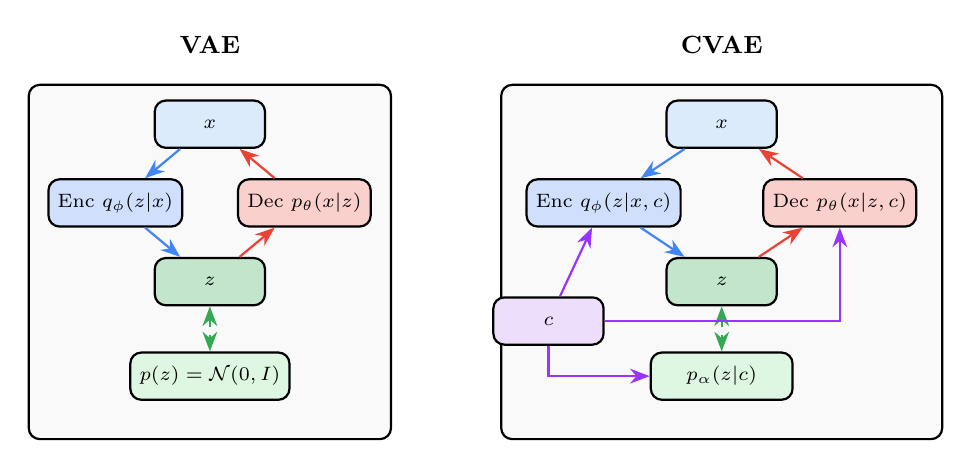
\begin{tikzpicture}[
    >={Stealth[length=2.5mm]},
    box/.style={draw, rounded corners, minimum width=1.4cm, minimum height=0.6cm, font=\scriptsize, thick},
    title/.style={font=\small\bfseries},
]
    % VAE side
    \node[title] at (0, 3.5) {VAE};
    \draw[thick, rounded corners, fill=gray!5] (-2.3, -1.5) rectangle (2.3, 3);

    \node[box, fill=lightblue] (vx) at (0, 2.5) {$x$};
    \node[box, fill=enccolor!25] (ve) at (-1.2, 1.5) {Enc $q_\phi(z|x)$};
    \node[box, fill=latentcolor!30] (vz) at (0, 0.5) {$z$};
    \node[box, fill=deccolor!25] (vd) at (1.2, 1.5) {Dec $p_\theta(x|z)$};
    \node[box, fill=lightgreen] (vp) at (0, -0.7) {$p(z) = \mathcal{N}(0,I)$};

    \draw[->, thick, enccolor] (vx) -- (ve);
    \draw[->, thick, enccolor] (ve) -- (vz);
    \draw[->, thick, deccolor] (vz) -- (vd);
    \draw[->, thick, deccolor] (vd) -- (vx);
    \draw[<->, thick, dashed, latentcolor] (vz) -- (vp);

    % CVAE side
    \node[title] at (6.5, 3.5) {CVAE};
    \draw[thick, rounded corners, fill=gray!5] (3.7, -1.5) rectangle (9.3, 3);

    \node[box, fill=lightblue] (cx) at (6.5, 2.5) {$x$};
    \node[box, fill=enccolor!25, minimum width=1.8cm] (ce) at (5, 1.5) {Enc $q_\phi(z|x,c)$};
    \node[box, fill=latentcolor!30] (cz) at (6.5, 0.5) {$z$};
    \node[box, fill=deccolor!25, minimum width=1.8cm] (cd) at (8, 1.5) {Dec $p_\theta(x|z,c)$};
    \node[box, fill=lightgreen, minimum width=1.8cm] (cp) at (6.5, -0.7) {$p_\alpha(z|c)$};
    \node[box, fill=lightpurple] (cc) at (4.3, 0.0) {$c$};

    \draw[->, thick, enccolor] (cx) -- (ce);
    \draw[->, thick, enccolor] (ce) -- (cz);
    \draw[->, thick, deccolor] (cz) -- (cd);
    \draw[->, thick, deccolor] (cd) -- (cx);
    \draw[<->, thick, dashed, latentcolor] (cz) -- (cp);
    \draw[->, thick, condcolor] (cc) -- (ce);
    \draw[->, thick, condcolor] (cc) |- (cp);
    \draw[->, thick, condcolor] (cc) -| (cd);
\end{tikzpicture}
\caption{Side-by-side comparison of VAE (left) and CVAE (right). The key difference: CVAE feeds condition $c$ to encoder, decoder, and optionally the prior.}
\label{fig:vae-vs-cvae}
\end{figure}

\begin{center}
\renewcommand{\arraystretch}{1.5}
\begin{tabular}{lcc}
\toprule
& \textbf{VAE} & \textbf{CVAE} \\
\midrule
Goal & Model $p(x)$ & Model $p(x|c)$ \\
Prior & $p(z) = \mathcal{N}(0,I)$ & $p_\alpha(z|c)$ (or $\mathcal{N}(0,I)$) \\
Encoder input & $x$ & $(x, c)$ \\
Decoder input & $z$ & $(z, c)$ \\
Latent $z$ captures & All variation in $x$ & Residual variation beyond $c$ \\
\midrule
ELBO & $\mathbb{E}_{q}[\log p(x|z)] - \mathrm{KL}(q\|p)$ & $\mathbb{E}_{q}[\log p(x|z,c)] - \mathrm{KL}(q\|p_c)$ \\
\bottomrule
\end{tabular}
\end{center}

\subsection{When to Use Which?}

\begin{itemize}
    \item \textbf{VAE}: No conditioning information available; want to learn the full data distribution $p(x)$.
    \item \textbf{CVAE}: Have auxiliary information $c$ and want controlled/conditional generation:
    \begin{itemize}
        \item Generate specific digit classes.
        \item Predict diverse futures given context.
        \item Conditional data augmentation.
    \end{itemize}
\end{itemize}

%% ============================================================
\section{Common Challenges and Solutions}
%% ============================================================

\subsection{Posterior Collapse}

\begin{figure}[H]
\centering
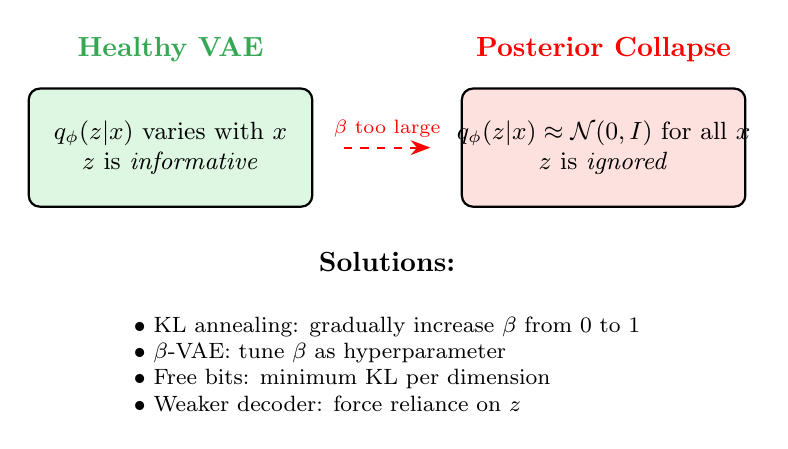
\begin{tikzpicture}[
    >={Stealth[length=2.5mm]},
    every node/.style={font=\small},
]
    % Normal case
    \node[font=\bfseries, latentcolor] at (0, 2.5) {Healthy VAE};
    \draw[thick, fill=lightgreen, rounded corners] (-1.8, 0.5) rectangle (1.8, 2);
    \node[align=center] at (0, 1.25) {$q_\phi(z|x)$ varies with $x$\\$z$ is \emph{informative}};

    % Collapsed case
    \node[font=\bfseries, red] at (5.5, 2.5) {Posterior Collapse};
    \draw[thick, fill=lightred, rounded corners] (3.7, 0.5) rectangle (7.3, 2);
    \node[align=center] at (5.5, 1.25) {$q_\phi(z|x) \approx \mathcal{N}(0,I)$ for all $x$\\$z$ is \emph{ignored}};

    % Arrow
    \draw[->, thick, red, dashed] (2.2, 1.25) -- node[above, font=\scriptsize] {$\beta$ too large} (3.3, 1.25);

    % Solutions
    \node[font=\bfseries] at (2.75, -0.2) {Solutions:};
    \node[align=left, font=\footnotesize] at (2.75, -1.5) {
        $\bullet$ KL annealing: gradually increase $\beta$ from 0 to 1\\
        $\bullet$ $\beta$-VAE: tune $\beta$ as hyperparameter\\
        $\bullet$ Free bits: minimum KL per dimension\\
        $\bullet$ Weaker decoder: force reliance on $z$
    };
\end{tikzpicture}
\caption{Posterior collapse: the encoder ignores input and outputs the prior for all $x$, making $z$ uninformative. Several remedies exist.}
\label{fig:collapse}
\end{figure}

\subsection{Blurry Samples}

VAE samples tend to be blurrier than GAN samples because:
\begin{itemize}
    \item Gaussian likelihood with MSE loss averages over modes.
    \item The approximate posterior may not capture the true posterior well.
\end{itemize}

\textbf{Solutions:} More expressive decoders, normalizing flows in latent space, or hybrid VAE-GAN models.

\subsection{The $\beta$-VAE Trade-off}

\begin{figure}[H]
\centering
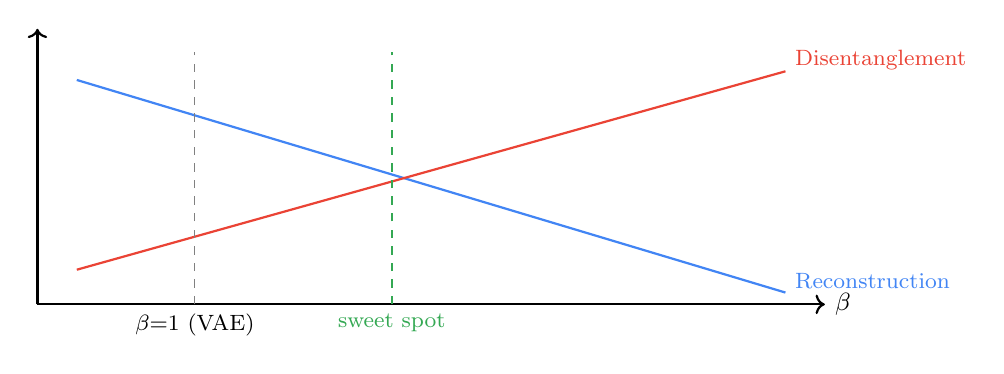
\begin{tikzpicture}[
    every node/.style={font=\small},
]
    % Axis
    \draw[->, thick] (0,0) -- (10,0) node[right] {$\beta$};
    \draw[->, thick] (0,0) -- (0,3.5);

    % Reconstruction quality curve
    \draw[thick, enccolor, domain=0.5:9.5, samples=50]
        plot (\x, {3 - 0.3*\x});
    \node[enccolor, right] at (9.5, 0.3) {\footnotesize Reconstruction};

    % Disentanglement curve
    \draw[thick, deccolor, domain=0.5:9.5, samples=50]
        plot (\x, {0.3 + 0.28*\x});
    \node[deccolor, right] at (9.5, 3.1) {\footnotesize Disentanglement};

    % beta = 1 marker
    \draw[dashed, gray] (2, 0) -- (2, 3.2);
    \node[below, font=\footnotesize] at (2, 0) {$\beta{=}1$ (VAE)};

    % Sweet spot
    \draw[dashed, latentcolor, thick] (4.5, 0) -- (4.5, 3.2);
    \node[below, font=\footnotesize, latentcolor] at (4.5, 0) {sweet spot};
\end{tikzpicture}
\caption{The $\beta$-VAE trade-off: increasing $\beta$ improves disentanglement but degrades reconstruction quality.}
\label{fig:beta-tradeoff}
\end{figure}

%% ============================================================
\section{Summary}
%% ============================================================

\begin{figure}[H]
\centering
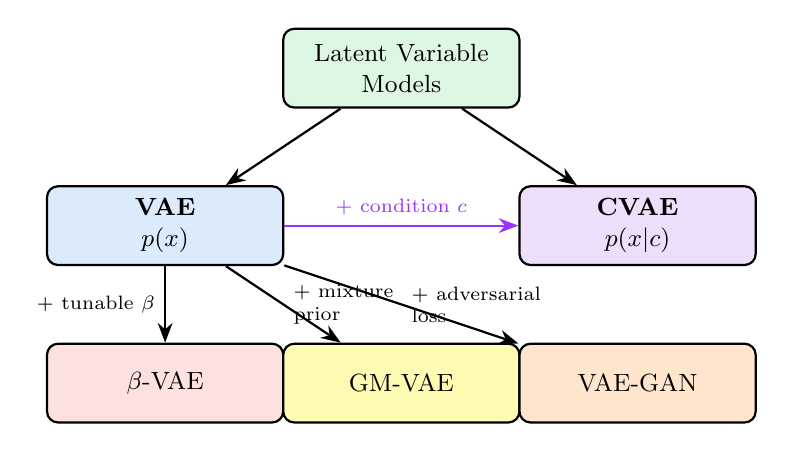
\begin{tikzpicture}[
    >={Stealth[length=2.5mm]},
    concept/.style={draw, rounded corners, thick, minimum width=3cm, minimum height=1cm, align=center, font=\small},
]
    \node[concept, fill=lightgreen] (lvm) at (0, 4) {Latent Variable\\Models};
    \node[concept, fill=lightblue] (vae) at (-3, 2) {\textbf{VAE}\\$p(x)$};
    \node[concept, fill=lightpurple] (cvae) at (3, 2) {\textbf{CVAE}\\$p(x|c)$};
    \node[concept, fill=lightred] (betavae) at (-3, 0) {$\beta$-VAE};
    \node[concept, fill=yellow!30] (gmvae) at (0, 0) {GM-VAE};
    \node[concept, fill=orange!20] (vaegan) at (3, 0) {VAE-GAN};

    \draw[->, thick] (lvm) -- (vae);
    \draw[->, thick] (lvm) -- (cvae);
    \draw[->, thick] (vae) -- node[left, font=\scriptsize] {$+$ tunable $\beta$} (betavae);
    \draw[->, thick] (vae) -- node[right, font=\scriptsize, align=left] {$+$ mixture\\prior} (gmvae);
    \draw[->, thick] (vae) -- node[right, font=\scriptsize, align=left] {$+$ adversarial\\loss} (vaegan);
    \draw[->, thick, condcolor] (vae) -- node[above, font=\scriptsize] {$+$ condition $c$} (cvae);
\end{tikzpicture}
\caption{The VAE family: VAE and CVAE are the two core frameworks, with many extensions.}
\label{fig:vae-family}
\end{figure}

\begin{itemize}
    \item \textbf{VAE} provides a principled framework for learning deep latent variable models by jointly training an encoder and decoder via the ELBO.
    \item The \textbf{reparameterization trick} enables end-to-end gradient-based optimization through stochastic sampling.
    \item \textbf{CVAE} extends VAE to conditional generation by incorporating condition $c$ into all components.
    \item Both models optimize a variational lower bound on the (conditional) log-likelihood.
\end{itemize}

\begin{thebibliography}{9}
\bibitem{kingma2014auto}
D.~P.~Kingma and M.~Welling.
\newblock Auto-Encoding Variational Bayes.
\newblock In \emph{ICLR}, 2014.

\bibitem{rezende2014stochastic}
D.~J.~Rezende, S.~Mohamed, and D.~Wierstra.
\newblock Stochastic Backpropagation and Approximate Inference in Deep Generative Models.
\newblock In \emph{ICML}, 2014.

\bibitem{sohn2015learning}
K.~Sohn, H.~Lee, and X.~Yan.
\newblock Learning Structured Output Representation using Deep Conditional Generative Models.
\newblock In \emph{NeurIPS}, 2015.

\bibitem{kingma2014semi}
D.~P.~Kingma, D.~J.~Rezende, S.~Mohamed, and M.~Welling.
\newblock Semi-Supervised Learning with Deep Generative Models.
\newblock In \emph{NeurIPS}, 2014.

\bibitem{higgins2017beta}
I.~Higgins, L.~Matthey, A.~Pal, C.~Burgess, X.~Glorot, M.~Botvinick, S.~Mohamed, and A.~Lerchner.
\newblock $\beta$-VAE: Learning Basic Visual Concepts with a Constrained Variational Framework.
\newblock In \emph{ICLR}, 2017.

\bibitem{kingma2016improved}
D.~P.~Kingma, T.~Salimans, R.~Jozefowicz, X.~Chen, I.~Sutskever, and M.~Welling.
\newblock Improved Variational Inference with Inverse Autoregressive Flow.
\newblock In \emph{NeurIPS}, 2016.
\end{thebibliography}

\end{document}
